% @Author: AnthonyKenny98
% @Date:   2020-04-09 12:52:23
% @Last Modified by:   AnthonyKenny98
% @Last Modified time: 2020-04-09 20:19:52
\begin{figure}[H]
\begin{centering}
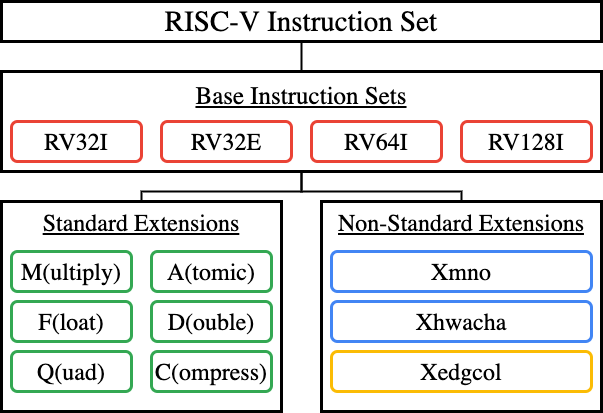
\includegraphics[width=0.8\linewidth]{chapters/chapter4/img/modules.png}
\mycaption{RISC-V ISA Modularity}{. It is clear that the RISC-V ISA is in fact a family of ISAs. Each is based on one of the ``base'' ISAs, which are each the smallest possible ISA to run just about any program. For more instructions and thus, better performance, any number of Standard or Non-Standard Extensions can be implemented on top of a base ISA.}
\label{fig:modules}
\end{centering}
\end{figure}